\documentclass[12pt]{article}
\usepackage[a4paper, margin=2.5cm]{geometry} % Set A4 paper size and margins
\usepackage{amsmath} % for mathematical symbols...
\usepackage{amsfonts} % for mathematical fonts
\usepackage[most]{tcolorbox}
\usepackage{tikz}


% Define a new quote environment with a nice box
\newtcolorbox{nicequote}{
    enhanced, % allows for advanced features
    colback=white, % background color
    colframe=black, % border color
    arc=0mm, % corner radius
    boxrule=0.5pt, % border width
    left=10pt, % left margin
    right=10pt, % right margin
}

\begin{document}

\section*{Osnovne algebrske strukture}

\subsection*{Algebrska struktura}

\textbf{Definicija 1.1} \\

\noindent
Naj bo $\mathbb{S}$ poljubna neprazna množica. \\
Vsaki preslikavi $\varphi : \mathbb{S} \times \mathbb{S} \to \mathbb{S}$ rečemo DVOMESTNA NOTRANJA OPERACIJA ali okrajšano DNO na množici $\mathbb{S}$. \\
Sliko urejenega para $(a, b) \in \mathbb{S} \times \mathbb{S}$ pišemo $a\varphi b$ (namesto običajnega zapisa $\varphi(a, b)$) in jo imenujemo KOMPOZITUM (SESTAV) ELEMENTOV $a$ in $b$ iz $\mathbb{S}$. \\
Dvomestno notranjo operacijo označujemo z znaki: $+, \cdot, \circ, \triangle, \heartsuit, \ldots$



\vspace{24pt}



\noindent
\textbf{Zgled 1.2} \\

\noindent
a) $\mathbb{S} = \mathbb{N}$ \\ 
\hspace*{1em} $\circ$ je običajno seštevanje naravnih števil. \\
\hspace*{1em} Sledi, je DNO, saj $\forall a, b \in \mathbb{N}$ je $a \circ b \in \mathbb{N}$. \\

\noindent
b) $\mathbb{S} = \mathbb{N}$ \\
\hspace*{1em} $\circ$ je običajno odštevanje naravnih števil. \\
\hspace*{1em} Sledi, ni DNO, npr.: za $1 \circ 2 = 1 - 2 = -1 \notin \mathbb{N}$.



%\begin{nicequote}
%    This is the quoted text. LaTeX will format it as a block quote with a nice box around it.
%\end{nicequote}



\vspace*{24pt}


\noindent
\textbf{Definicija 1.3} \\

\noindent
DNO $\circ$ na množici $\mathbb{S} \ne \emptyset$ je ASOCIATIVNA če za vse elemente
$a, b, c \in \mathbb{S}$ velja
$$(a \circ b) \circ c = a \circ (b \circ c)$$
KOMUTATIVNA, če za vsaka elementa $a, b \in \mathbb{S}$ velja
$$a \circ b = b \circ a$$



\vspace*{24pt}


\noindent
\textbf{Zgled 1.4.} \\

\noindent
a) $\mathbb{S} = \mathbb{Z}$ \\
\hspace*{1em} $\circ$ je običajno seštevanje celih števil. \\
\hspace*{1em} Sledi, je DNO. \\
\hspace*{1em} Sledi, $\circ$ je komutativna, in je asociativna. \\

\noindent
b) $\mathbb{S} = \mathbb{Z}$ \\
\hspace*{1em} $\circ$ je odštevanje celih števil. \\
\hspace*{1em} Sledi, je DNO. \\
\hspace*{1em} Preverimo komutativnost:
\begin{align*}
    a &= 1, b = 0 \\
    a \circ b &= 1 - 0 = 1 \\
    b \circ a &= 0 - 1 = -1    
\end{align*}
\hspace*{1em} Sledi, ni komutativno.

\noindent
\hspace*{1em} Preverimo, asociativnost:
\begin{align*}
    a = 1, b &= 2, c = 3 \\
    (a \circ b) \circ c = & (1 - 2) - 3 = -4 \\
    a \circ (b \circ c) = & 1 - (2 - 3) = 2
\end{align*}
\hspace*{1em} Sledi, ni asociativno. \\

\noindent
c) $\mathbb{S} = \mathbb{R}^{n \times n}$ (kvadratne matrike z realnimi koeficienti) \\
\hspace*{1em} $\circ$ je običajno množenje matrik. \\
\hspace*{1em} Sledi, je DNO, ker je rezultat zmnožka spet kvadratna matrika velikosti $n \times n$ z realnimi \\
\hspace*{1em} koeficienti. \\
\hspace*{1em} Preverimo asociativnost: \\
\begin{align*}
    A = 
    \begin{bmatrix}
        a_1 & b_1 \\
        c_1 & d_1 \\
    \end{bmatrix}, 
    B = &
    \begin{bmatrix}
        a_2 & b_2 \\
        c_2 & d_2 \\
    \end{bmatrix},
    C = 
    \begin{bmatrix}
        a_3 & b_3 \\
        c_3 & d_3 \\
    \end{bmatrix} \\
\end{align*}
\begin{align*}
    (A \circ B) \circ C &= 
        \left(
            \begin{bmatrix}
                a_1 & b_1 \\
                c_1 & d_1 \\               
            \end{bmatrix}
            \cdot
            \begin{bmatrix}
                a_2 & b_2 \\
                c_2 & d_2 \\
            \end{bmatrix}
        \right)
        \cdot
        \begin{bmatrix}
            a_3 & b_3 \\
            c_3 & d_3 \\
        \end{bmatrix}
        \\[1em]
        & =
        \begin{bmatrix}
            a_1a_2 + b_1c_2 & a_1b_2 + b_1d_2 \\ 
            c_1a_2 + d_1c_2 & c_1b_2 + d_1d_2 \\
        \end{bmatrix}
        \cdot
        \begin{bmatrix}
            a_3 & b_3 \\
            c_3 & d_3 \\
        \end{bmatrix}
        \\[1em]
        & = 
        \begin{bmatrix}
            (a_1a_2 + b_1c_2)a_3 + (a_1b_2 + b_1d_2)c_3 & (a_1a_2 + b_1c_2)b_3 + (a_1b_2 + b_1d_2)d_3 \\ 
            (c_1a_2 + d_1c_2)a_3 + (c_1b_2 + d_1d_2)c_3 & (c_1a_2 + d_1c_2)b_3 + (c_1b_2 + d_1d_2)d_3 \\ 
        \end{bmatrix}
        \\[1em]
        & = 
        \begin{bmatrix}
            a_1a_2a_3 + b_1a_3c_2 + a_1c_2c_3 + b_1c_3d_2 & a_1a_2b_3 + b_1b_2d_3 + a_1b_2c_3 + b_1c_2d_3 \\ 
            c_1a_2a_3 + d_1a_3c_2 + c_1c_2c_3 + d_1c_3d_2 & c_1a_2b_3 + d_1b_2d_3 + c_1b_2c_3 + d_1c_2d_3 \\
        \end{bmatrix}
\end{align*}

\begin{align*}
    A \circ (B \circ C) 
    &=
    \begin{bmatrix}
        a_1 & b_1 \\
        c_1 & d_1 \\
    \end{bmatrix} 
    \cdot 
    \left(
        \begin{bmatrix}
            a_2 & b_2 \\
            c_2 & d_2 \\
        \end{bmatrix} 
        \cdot
        \begin{bmatrix}
            a_3 & b_3 \\
            c_3 & d_3 \\
        \end{bmatrix} 
    \right)
    \\[1em]
    &=
    \begin{bmatrix}
        a_1 & b_1 \\
        c_1 & d_1 \\
    \end{bmatrix} 
    \cdot 
    \begin{bmatrix}
        a_2a_3+b_2c_3 & a_2b_3+b_2d_3 \\
        c_2a_3 + d_2c_3 & c_2b_3+d_2d_3 \\
    \end{bmatrix}
    \\[1em]
    &=
    \begin{bmatrix}
        a_1(a_2a_3+b_2c_3) + b_1(c_2a_3 + d_2c_3) & a_1(a_2b_3+b_2d_3) + b_1(c_2b_3+d_2d_3) \\
        c_1(a_2a_3+b_2c_3) + d_1(c_2a_3 + d_2c_3) & c_1(a_2b_3+b_2d_3) + d_1(c_2b_3+d_2d_3) \\
    \end{bmatrix}
    \\[1em]
    &=
    \begin{bmatrix}
        a_1a_2a_3 + b_1a_3c_2 + a_1c_2c_3 + b_1c_3d_2 & a_1a_2b_3 + b_1b_2d_3 + a_1b_2c_3 + b_1c_2d_3 \\
        c_1a_2a_3 + d_1a_3c_2 + c_1c_2c_3 + d_1c_3d_2 & c_1a_2b_3 + d_1b_2d_3 + c_1b_2c_3 + d_1c_2d_3 \\
    \end{bmatrix}
\end{align*}
\hspace*{1em} Sledi, je asociativno.

\noindent
\hspace*{1em} Preverimo komutativnost: \\
\begin{align*}
    A = 
    \begin{bmatrix}
        1 & 1 \\
        1 & 1 \\
    \end{bmatrix}, 
    B = 
    \begin{bmatrix}
        1 & 1 \\
        0 & 0 \\
    \end{bmatrix}
\end{align*}

\begin{align*}
    A \circ B = 
    \begin{bmatrix}
        1 & 1 \\
        1 & 1 \\
    \end{bmatrix} \cdot 
    \begin{bmatrix}
        1 & 1 \\
        0 & 0 \\
    \end{bmatrix}
    = 
    \begin{bmatrix}
        1 & 1 \\
        1 & 1 \\
    \end{bmatrix}
\end{align*}

\begin{align*}
    B \circ A = 
    \begin{bmatrix}
        1 & 1 \\
        0 & 0 \\
    \end{bmatrix} \cdot 
    \begin{bmatrix}
        1 & 1 \\
        1 & 1 \\
    \end{bmatrix} =
    \begin{bmatrix}
        2 & 2 \\
        0 & 0 \\
    \end{bmatrix}
\end{align*}



\vspace*{24pt}


\noindent
\textbf{Trditev 1.5.} \\
Če je DNO $\circ$ na $\mathbb{S} \ne \emptyset$ asociativna, potem je produkt (kompozitum) elementov \\
$a_1, a_2, ..., a_n \in \mathbb{S}$ $(n \in \mathbb{N})$ natančno določen z vrstnim redom teh elementov. \\
Tak produkt označimo z $a_1 \circ a_2 \circ \dots \circ a_n$. \\
Dokaz: izpustimo!




\vspace*{24pt}


\noindent
\textbf{Trditev 1.6.} \\
Če je $\circ$ asociativna in komutativna DNO na $\mathbb{S} \ne \emptyset$, potem je naš produkt elementov \\
$a_1, a_2, \dots, a_n \in \mathbb{S}$ $(n \in \mathbb{N})$ enolično določen ne glede na vrstni red naših elementov. \\
Dokaz: izpustimo!




\vspace*{24pt}


\noindent
\textbf{Definicija 1.7.} \\
Naj bo $\mathbb{S} \ne \emptyset$ z DNO $\circ$. \\
Element $l \in \mathbb{S}$ je LEVI NEUTRALNI ELEMENT v množici $\mathbb{S}$, če za $\forall a \in \mathbb{S}$ velja
$$l \circ a = a$$
Element $d \in \mathbb{S}$ je DESNI NEUTRALNI ELEMENT v množici $\mathbb{S}$, če za $\forall a \in \mathbb{S}$ velja
$$a \circ d = a$$
Če je $e \in \mathbb{S}$ hkrati levi in desni neutralni element v množici $\mathbb{S}$, mu preprosto rečemo \\
NEUTRALNI ELEMENT. \\
Oznaka: $(\mathbb{S}, \circ)$ \dots neprazna množica $\mathbb{S}$ z DNO.


\vspace*{24pt}


\noindent
\textbf{Trditev 1.8.} \\
Če $(\mathbb{S}, \circ)$ premore levi in desni neutralni element, potem sta enaka. \\
Dokaz: \\
Naj bo $l \in \mathbb{S}$ levi neutralni element in $d \in \mathbb{S}$ desni neutralni element v množici $\mathbb{S}$, potem:
$$l = l \circ d = d$$
Torej sklepamo, da je $l = d$, kar smo želeli pokazati.



\vspace*{24pt}


\noindent
\textbf{Zgled 1.9.} \\

\noindent
a) $S = \mathbb{R}^{2 \times 2} = \{ 
    \begin{bmatrix} 
        a & b \\
        c & d \\
    \end{bmatrix}
    ; a, b, c, d \in \mathbb{R}
\}$ \\
\hspace*{1em} $\circ$ je običajno množenje matrik. \\
\hspace*{1em} Sledi, je DNO.\\
\hspace*{1em} $I = \begin{bmatrix}
    1 & 0 \\
    0 & 1 \\
\end{bmatrix}$ je neutralni element, saj za $\forall A \in S$ velja $I \cdot A = A \cdot I = A$. \\

\noindent
b) $S = \{
    \begin{bmatrix}
        a & b \\
        0 & 0 \\
    \end{bmatrix}
    \}; a, b \in \mathbb{R}$ \\
\hspace*{1em} $\circ$ je običajno množenje matrik. \\
\hspace*{1em} $
    \begin{bmatrix}
        a & b \\
        0 & 0 \\
    \end{bmatrix}
    \cdot
    \begin{bmatrix}
        x & y \\
        0 & 0 \\
    \end{bmatrix}
    =
    \begin{bmatrix}
        ax & ay \\
        0 & 0 \\
    \end{bmatrix}
$ \\
\hspace*{1em} Sledi, je DNO.
\hspace*{1em} Levi neutralni element:

\begin{align*}
    \begin{bmatrix}
        ax & ay \\
        0 & 0 \\
    \end{bmatrix}
    &= 
    \begin{bmatrix}
        x & y \\
        0 & 0 \\
    \end{bmatrix} \\
    &\Downarrow \\
    a = 1, b &= \text{ poljuben } \\
    &\Downarrow \\
    \forall b \in \mathbb{R} \text{ je }
    \begin{bmatrix}
        1 & b \\
        0 & 0 \\    
    \end{bmatrix} &
    \text{ levi neutralni element v } S
\end{align*} \\

\noindent
\hspace*{1em} Desni neutralni element: \\

\begin{align*}
    \begin{bmatrix}
        ax & ay \\
        0 & 0 \\
    \end{bmatrix}
    &= 
    \begin{bmatrix}
        a & b \\
        0 & 0 \\
    \end{bmatrix} \\
    & \Downarrow \\
    ax = a & \Rightarrow x = 1 \\
    ay = b & \Rightarrow y = \frac{b}{a} \text{ ni OK! Ker je odvisno od } a, b. \\
    & \Downarrow \\
    \text{ desni neutralni } & \text{element ne obstaja!}
\end{align*}



\vspace*{24pt}


\noindent
\textbf{Definicija 1.10.} \\
Naj $(S, \circ)$ premore neutralni element $e \in S$, ter naj bo $a \in S$ poljuben. \\
Potem $l \in S$ je LEVI OBRAT (ali INVERZ) ELEMENTA $a \in S$ če velja \\
$$l \circ a = e$$
Element $d \in S$ je DESNI OBRAT ELEMENTA $a \in S$ če velja \\
$$a \circ d = e$$
OBRAT ELEMENTA $a \in S$ je tak element iz $S$ ki je hkrati levi in desni obrat od $a$. \\

\noindent
Element $a \in S$ je obrnljiv (v množici $S$) če premore obrat v množici $S$. \\



\vspace*{24pt}


\noindent
\textbf{Trditev 1.11.} \\
Naj veljajo oznake iz definicije 1.10. \\
Neutralni element $e$ je obrat samega sebe. \\
Dokaz:
$$e \circ e = e$$



\vspace*{24pt}


\noindent
\textbf{Trditev 1.12.} \\
Naj bo $S \ne \emptyset$ z DNO $\circ$, ki je asociativna in naj bo $e \in S$ neutralni element. \\
Če ima element $a \in S$ levi in desni obrat v $S$, potem sta enaka. \\[1em]
Dokaz:
Naj veljajo predpostavke iz trditve 1.12. in $a \in S$. \\
$$ \exists \text{levi obrat za } a \text{ v } S \Rightarrow \exists l \in S: l \circ a = e $$
$$ \exists \text{desni obrat za } a \text{ v } S \Rightarrow \exists d \in S: a \circ d = e $$
Potem je
$$ (l \circ a) \circ d = e \circ d = d $$
$$ l \circ (a \circ d) = l \circ e = l $$
ker je $\circ$ asociativna operacija. \\
Torej, je $l = d$.



\vspace*{24pt}


\noindent
\textbf{Definicija 1.13.} \\
Če je $S \ne \emptyset$ z DNO $\circ$, ki je asociativna, potem rečemo, da je $(S, \circ)$ POLGRUPA. \\
Polgrupa z neutralnim elementom je MONOID. \\
Monoid v katerem je vsak element obrnljiv je GRUPA. \\

\begin{tabular}{|c|c|c|c|}
    \hline
    $(S, \circ)$ & $\circ$ asociativna & $\exists$ neutralen element & $\forall a \in S$ je obrnljiv \\
    \hline
    POLGRUPA & $\checkmark$ & $\times$ & $\times$ \\
    \hline
    MONOID & $\checkmark$ & $\checkmark$ & $\times$ \\
    \hline
    GRUPA & $\checkmark$ & $\checkmark$ & $\checkmark$ \\
    \hline
\end{tabular}



\vspace*{24pt}


\noindent
\textbf{Definicija 1.14.} \\
Če izbrano DNO na $S \ne \emptyset$ označimo s +, potem govorimo o SEŠTEVAJOČEM \\
(ali ADITIVNEM) ZAPISU. \\
Element $a + b$ je VSOTA elementov $a, b \in S$, neutralni element označimo z $0 \in S$ \\
(in mu rečemo ničla), obratu elementa $a \in S$ rečemo NASPROTNI ELEMENT in ga \\
označimo z $-a$. \\[1em]

\noindent
Če izbrano DNO na $S \in \emptyset$ označimo z $\cdot$, potem govorimo o MNOŽEČEM \\
(ali MULTIPLIKATIVNEM) ZAPISU.
$$a \cdot b = ab$$ \\[1em]

\noindent
Element $ab$ je zmnožek (ali PRODUKT) elementa $a, b \in S$, neutralni element označimo \\
z $1 \in S$ (in mu rečemo enka), obrat elementa $a \in S$ rečemo INVERZ, označimo z $a^{-1}$. \\



\noindent
\textbf{Definicija 1.15.} \\
Naj bo $\Omega \ne \emptyset$. \\
$Map(\Omega) = \{ f : \Omega \to \Omega \}$ $\leftarrow$ množica vseh preslikav iz $\Omega$ v $\Omega$. \\
Množico $Map(\Omega)$ opremimo z (običajno) operacijo levega sestavljanja preslikav:
$$
\forall f, g : \Omega \to \Omega \text{ je } f \circ g : \Omega \to \Omega
$$ 
$$
\text{in } \forall x \in \Omega \text{ velja } (f\circ g)(x) = f(g(x))
$$\\[2em]

\noindent
Operacija $\circ$ iz definicije 1.15 je DNO na $Map(\Omega)$.



\vspace*{24pt}


\noindent
\textbf{Trditev 1.16.} \\
$(Map(\Omega), \circ)$ je monoid. \\[1em]
Dokaz: \\[1em]
$I)$ $\circ$ je asociativna. (moramo dokazati, oz. dokazano spodaj)
$$
\forall f, g, g \in Map(\Omega) : (f \circ g) \circ h = f \circ (g \circ h)
$$
Opazimo:
$$
((f \circ g) \circ h)(x) = f(g(h(x)))
$$
$$
(f\circ (g \circ h))(x) = f(g(h(x)))
$$
\\[1em]

\noindent
$II)$ $\exists$ neutralnega elementa v $Map(\Omega)$ za $\circ$
$$
\forall x \in \Omega \text{ naj bo } id : x \to x \text{ (identična preslikava)}
$$
$$
\text{Pogazati moramo: } \forall f \in Map(\Omega): f \circ id = id \circ f = features
$$
\begin{align*}
    \forall x \Omega \text{ velja: } & (f \circ id)(x) = f(id(x)) = f(x) \\
    & (id \circ f)(x) = id(f(x)) = f(x)
\end{align*}



\vspace*{24pt}


\noindent
\textbf{Definicija 1.15.} (nadaljevanje) \\
Podobno definiramo: 
$$Inj(\Omega) = \{ f: \Omega \to \Omega ; f \text{ je injektivna }\}$$
$$Sur(\Omega) = \{ f: \Omega \to \Omega ; f \text{ je surjektivna } \}$$
$$Bij(\Omega) = \{ f: \Omega \to \Omega ; f \text{ je bijektivna } \}$$
in jih opremimo z operacijo sestavljanja preslikav z istim predpisom.



\vspace*{24pt}


\noindent
\textbf{Trditev 1.17.} \\
$(Inj(\Omega), \circ)$ in $(Sur(\Omega), \circ)$ sta monoida, $(Bij(\Omega), \circ)$ je grupa. \\[1em]
Dokaz: D.N. (za domačo nalogo)



\vspace*{24pt}


\noindent
\textbf{Trditev 1.18.} \\
Naj bo $(A, \cdot)$ polgrupa z neutralnim elementom in naj bo 
$$a_1, a_2, \dots, a_n \in A \text{ } (n \in \mathbb{N}) \text{ obrnljivi.}$$
Potem velja: produkt $a_1, a_2, \dots, a_n$ je obrnljiv in njegov obrat je 
$$(a_1, a_2, \dots, a_n)^{-1} = a_n^{-1}, \dots, a_2^{-1}, a_1^{-1}$$
Dokaz: Indukcija po $n$: \\
$n = 2$; Naj bosta $a_1, a_2 \in A$ obrnljiva
\begin{align*}
    (a_1a_2)\cdot (a_1a_2)^{-1} &= a_1 \cdot a_2 \cdot a_2^{-1} \cdot a_1^{-1} = a_1 \cdot 1 \cdot a_1^{-1} = a_1a_1^{-1} = 1 \\
    (a_1a_2)^{-1} \cdot (a_1a_2) &= \dots \text{ podobno }
\end{align*}
$n = n + 1$; D.N. (za domačo nalogo)



\vspace*{24pt}


\noindent
\textbf{Definicija 1.19.} \\
Naj bo $(A, \cdot)$ polgrupa z neutralnim elementom. \\
Za $\forall a \in A$ in $\forall n \in \mathbb{N}$ definirajmo POTENCO $a^n$ kot
\begin{align*}
    a^1 &= a \\
    a^2 &= a \cdot a \\
    &\phantom{=} \vdots \\
    a^{n+1} &= a^n \cdot a = a \cdot a \cdot a \dots a 
\end{align*}
Dodatno definirajmo, $a^0 = 1$. \\
Če je element $a \in A$ obrnljiv definiramo
$$
\forall n \in \mathbb{N} \text{ } \text{ } \text{ } \text{ } a^{-n} = a^{(-1)n} = (a^{-1})^n
$$



\vspace*{24pt}


\noindent
\textbf{Izrek 1.20.} (Adicijski izrek) \\
Naj bo $(A, \cdot)$ polgrupa z neutralnim elementom in naj bosta $m, n \in \mathbb{N}_0$. \\
Potem $\forall a \in A$ velja $a^{m + n} = a^m \cdot a^n$ \\
Če je $a \in A$ obrnljiv, velja adicijski izrek $\forall m, n \in \mathbb{Z}$.



\vspace*{24pt}


\noindent
\textbf{Definicija 1.21.} \\
Naj bo $(A, \cdot)$ polgrupa z neutralnim elementom. \\
Element $a \in A$ ima KONČEN RED, če obstaja $n \in \mathbb{N}$, da je $a^n = 1$. \\
V tem primeru najmanjšem številu $r \in \mathbb{N}$ za katerega je $a^r = 1$, rečemo \\
RED ELEMENTA $a$. \\[1em]
opomba 1: $|a|$ (red elementa $a$) \\
opomba 2: v primeru $(A, +)$ $a^n \to na$ in $1 \to 0$



\vspace*{24pt}


\noindent
\textbf{Zgled 1.22.} \\[1em]
a)  $A = \mathbb{Z} \backslash \{ 0 \}$ \\
\hspace*{1em} $\cdot$ je običajno množenje celih števil $\implies$ $(\mathbb{Z} \backslash \{0\}, \cdot)$ 
\begin{align*}
    1 \in \mathbb{Z} \backslash \{0\} &: 1^1 = 1, 1^2 = 1, 1^3 = 1, \dots \text{ element 1 ima končen red, red elementa 1 je 1} \\
    2 \in \mathbb{Z} \backslash \{0\} &: 2^1 = 2, 2^2 = 2 \cdot 2 = 4, 2^3 = 2 \cdot 2 \cdot 2 = 8, \dots \text{ nima končnega reda}
\end{align*}
Torej, števila večja od 1 nimajo končnega reda.
\begin{align*}
    -1 \in \mathbb{Z} \backslash \{0\} &: (-1)^1 = -1, (-1)^2 = (-1) \cdot (-1) = 1 \text{ red elementa -1 je 2}
\end{align*} \\

\noindent
b) $A = S^1 = \{ z \in \mathbb{C}; |z| = 1 \}$ \\
\hspace*{1em} $\cdot$ običajno množenje kompleksnih števil.
\begin{center}
    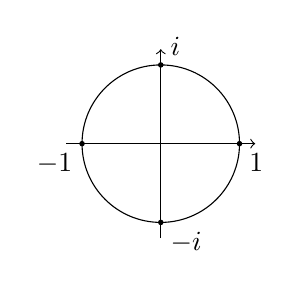
\begin{tikzpicture}
      \draw (0,0) circle [radius=1];
      \draw[->] (-1.2,0) -- (1.2,0);
      \draw[->] (0,-1.2) -- (0,1.2);
      \fill (1,0) circle[radius=1pt] node[below right] {$1$};
      \fill (-1,0) circle[radius=1pt] node[below left] {$-1$};
      \fill (0,1) circle[radius=1pt] node[above right] {$i$};
      \fill (0,-1) circle[radius=1pt] node[below right] {$-i$};
    \end{tikzpicture}
\end{center}
$$
0 + 1i = i \in S^1: i^1 = i, i^2 = -1, i^3 = -i, i^4 = 1 \text{ red elementa } i \text{ je 4}
$$
\begin{align*}
    -i \in S^1: (-i)^1 &= -i, (-i)^2 = (-i) \cdot (-i) = -1 \\
    (-i)^3 &= (-i)^1 \cdot (-i)^2 = -i \cdot (-1) = i \\
    (-i)^4 &= (-i)^2 \cdot (-i)^2 = (-1) \cdot (-1) = 1 \text{ red elementa } -i \text{ je 4}
\end{align*} \\

\noindent
c) $A = \mathbb{Z}$














\end{document}
